\section{Results}
\label{sec:results}

\subsection{Read: tokens}

\begin{figure}[t]
\centering
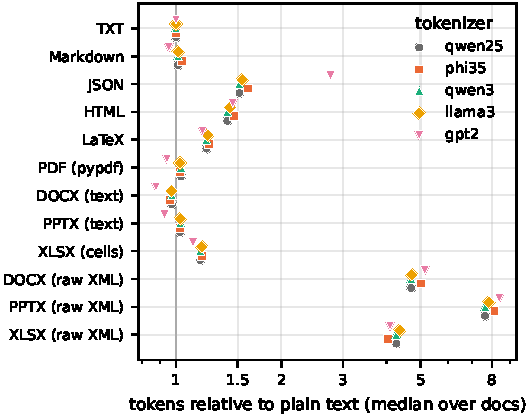
\includegraphics[width=\columnwidth]{figures_full/tokens.pdf}
\caption{Tokens per format relative to the plain-text version of the same
document (median over \NDocs{} documents), under five tokenizers.}
\label{fig:tokens}
\end{figure}

\begin{table}[t]
\centering
\caption{Read cost under the Qwen2.5 tokenizer. Density is
tokens(TXT)/tokens(format). Fixed and per-TXT-token are the intercept and
slope of tokens(format) $= a + b\cdot$tokens(TXT) over the size sweep.
Loader is the time to turn the file into a string.}
\label{tab:overhead}
\resizebox{\columnwidth}{!}{\begin{tabular}{lrrrrr}
\toprule
Format & tokens/TXT & density & loader (ms) & fixed & per TXT tok \\
\midrule
TXT & 1.00 & 100\% & -- & -0 & 1.00 \\
Markdown & 1.01 & 99\% & -- & 4 & 1.01 \\
JSON & 1.52 & 66\% & -- & 73 & 1.41 \\
HTML & 1.40 & 71\% & -- & 200 & 1.10 \\
LaTeX & 1.22 & 82\% & -- & 127 & 1.03 \\
PDF (pypdf) & 1.03 & 97\% & 22.0 & -24 & 1.07 \\
DOCX (text) & 0.97 & 103\% & 8.3 & -18 & 1.00 \\
PPTX (text) & 1.03 & 97\% & 5.6 & -12 & 1.05 \\
XLSX (cells) & 1.17 & 85\% & 3.0 & 64 & 1.08 \\
DOCX (raw XML) & 4.70 & 21\% & 0.2 & 2028 & 1.59 \\
PPTX (raw XML) & 7.65 & 13\% & 0.4 & 1946 & 4.65 \\
XLSX (raw XML) & 4.26 & 23\% & 0.2 & 1276 & 2.30 \\
\bottomrule
\end{tabular}
}
\end{table}

Figure~\ref{fig:tokens} and Table~\ref{tab:overhead} give the read cost.
The formats fall into three groups:
\begin{itemize}
\item \textbf{Extracted text costs what plain text costs.} The text that
  pypdf, python-docx, python-pptx and openpyxl extract is within a few
  percent of TXT. Markdown adds 1\,\%.
\item \textbf{Markup costs 1.2--1.5$\times$.} LaTeX costs
  \TokRatioTex$\times$, HTML \TokRatioHtml$\times$ and JSON
  \TokRatioJson$\times$. The cost model separates them. HTML's overhead is
  mostly fixed (\FixedHtml{} tokens of head and tags; slope
  \SlopeHtml). JSON's grows with content (slope \SlopeJson): every string
  brings quotes, a key and indentation. Under GPT-2's tokenizer, which has
  no tokens for runs of spaces, JSON costs about 2.8$\times$.
\item \textbf{Raw office XML costs 4--8$\times$.} DOCX XML costs
  \TokRatioDocxXml$\times$, XLSX XML \TokRatioXlsxXml$\times$ and PPTX XML
  \TokRatioPptxXml$\times$ (\PptxXmlRatioMin--\PptxXmlRatioMax{} across
  tokenizers). The slide XML's slope is \SlopePptxXml: each word of
  content arrives wrapped in run, paragraph and shape elements.
\end{itemize}
Loading is cheap next to reading: pypdf takes \LoaderPdfText\,ms per
document, while the model's prefill takes about a second.

\subsection{Understand: accuracy}

\begin{figure*}[t]
\centering
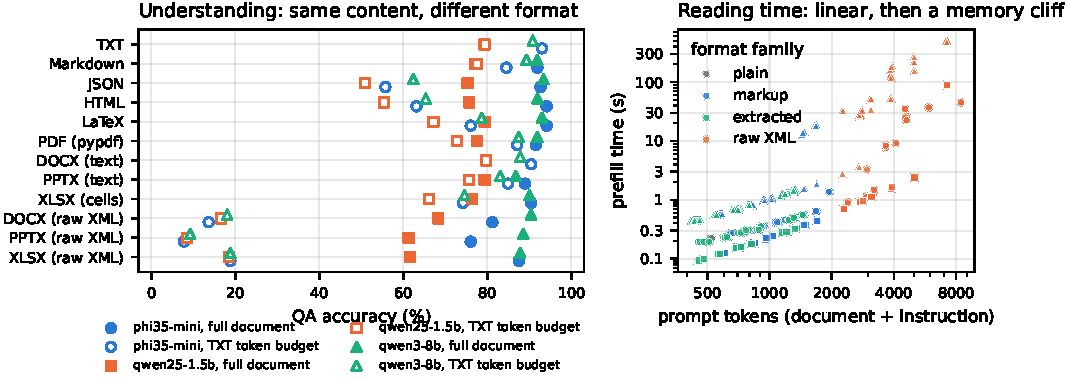
\includegraphics[width=\textwidth]{figures_full/understand.pdf}
\caption{Left: QA accuracy per read format, with the full document
(filled) and with the document cut to its plain-text token count (open).
Right: prefill time against prompt length, one point per
(document, format). Each family of points is linear until the prompt no
longer fits in GPU memory, then rises steeply.}
\label{fig:understand}
\end{figure*}

\begin{table}[t]
\centering
\caption{QA accuracy (\%) with the full document and at the plain-text
token budget, over \NDocs{} documents and about \NQuestionsPerDoc{}
questions each.}
\label{tab:accuracy}
\resizebox{\columnwidth}{!}{\begin{tabular}{lrrrrrr}
\toprule
Format & \multicolumn{2}{c}{phi35-mini} & \multicolumn{2}{c}{qwen25-1.5b} & \multicolumn{2}{c}{qwen3-8b} \\
 & full & budget & full & budget & full & budget \\
\midrule
TXT & 93 & 93 & 79 & 79 & 91 & 91 \\
Markdown & 92 & 85 & 77 & 77 & 92 & 89 \\
JSON & 93 & 56 & 75 & 51 & 93 & 62 \\
HTML & 94 & 63 & 76 & 55 & 92 & 65 \\
LaTeX & 94 & 76 & 79 & 67 & 93 & 79 \\
PDF (pypdf) & 92 & 87 & 77 & 73 & 92 & 87 \\
DOCX (text) & 90 & 90 & 80 & 80 & 88 & 88 \\
PPTX (text) & 89 & 85 & 79 & 76 & 87 & 83 \\
XLSX (cells) & 90 & 74 & 76 & 66 & 90 & 75 \\
DOCX (raw XML) & 81 & 14 & 68 & 17 & 90 & 18 \\
PPTX (raw XML) & 76 & 8 & 61 & 8 & 89 & 9 \\
XLSX (raw XML) & 87 & 19 & 62 & 18 & 88 & 19 \\
\bottomrule
\end{tabular}
}
\end{table}

\paragraph{With the whole document, format barely matters to the larger
model.} Qwen3-8B answers \AccMd\,\% from Markdown and between
\AccPptxText\,\% and \AccJson\,\% from every other format, raw XML
included (Figure~\ref{fig:understand}, Table~\ref{tab:accuracy}). After
Holm correction no format differs from Markdown (smallest adjusted
$p=$\,\MinPVsMd). The smaller models do notice raw XML. Qwen2.5-1.5B drops
from 77\,\% on Markdown to 61--68\,\% on the three XML forms, and
Phi-3.5-mini from 92\,\% to 76--87\,\%, while it scores 89--94\,\% on
every text and extracted form.

\paragraph{At a fixed budget, markup costs answers.} When each format gets
only as many tokens as the plain text, Markdown keeps \AccBudgetMd\,\%.
LaTeX falls to \AccBudgetTex\,\%, HTML to \AccBudgetHtml\,\%, JSON to
\AccBudgetJson\,\%, and raw XML to \AccXmlBudgetMean\,\% on average. Most of
that loss is content that no longer fits. But not all of it: among
questions whose answer string is still inside the cut context, Qwen3-8B
answers \AccBudgetEvidencePlain\,\% from TXT and Markdown and
\AccBudgetEvidenceXml\,\% from raw XML. Markup dilutes the content it does
not push out.

\paragraph{The memory cliff.} Prefill time grows linearly with tokens,
\PrefillMsPerKtok\,ms per thousand tokens for Qwen3-8B ($R^2=$\,\PrefillRsq),
until it doesn't (Figure~\ref{fig:understand}, right). Above
\CliffTokensQwenThreeEightb{} prompt tokens for Qwen3-8B,
\CliffTokensPhiThreeFiveMini{} for Phi-3.5-mini and
\CliffTokensQwenTwoFiveOneFiveb{} for Qwen2.5-1.5B, the time per token
jumps, up to \CliffSlowdown$\times$ the plain-text rate. The GPU has run
out of memory, and the Windows driver spills to system RAM instead of
failing. The one out-of-memory error we hit came from the attention call
asking for 10.8\,GiB at once, which suggests the attention matrix is
materialized in full and grows with the square of the prompt. The prompts past
the cliff are almost all raw XML and JSON. The median raw-PPTX prompt took
\PrefillXmlOverTxt$\times$ as long to read as its TXT version, where the
token ratio alone predicts \TokRatioPptxXml$\times$. The cliff depends on
the stack (GPU memory, attention kernel, driver), but the mechanism is
general: markup moves a document toward whatever memory limit the
hardware has.

\subsection{Write: the format tax}

\begin{figure*}[t]
\centering
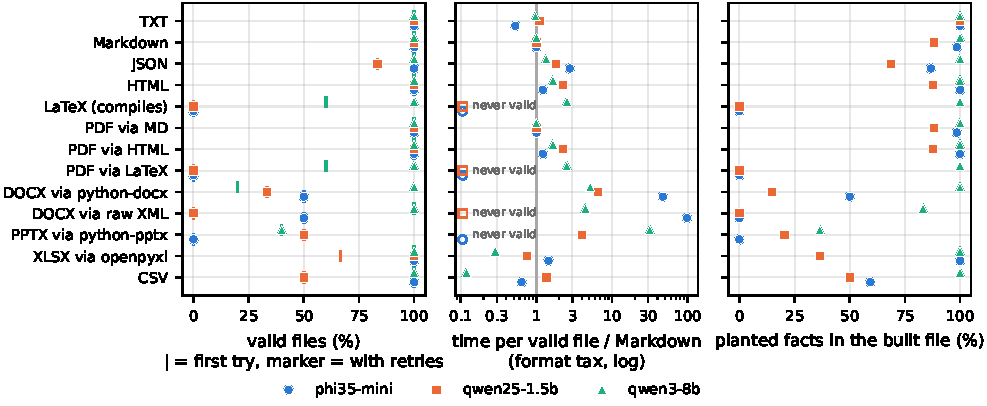
\includegraphics[width=\textwidth]{figures_full/write.pdf}
\caption{Writing each deliverable. Left: share of valid files, after
retries (marker) and on the first try (bar). Middle: time per valid file
relative to Markdown, the format tax (log scale). Right: planted facts that
survive in the built file.}
\label{fig:write}
\end{figure*}

\begin{table*}[t]
\centering
\caption{Writing: valid files (\%), median output tokens over all attempts,
format tax (time per valid file / Markdown) and planted facts recovered
from the built file (\%). Up to \MaxAttempts{} attempts, the build error
fed back each time.}
\label{tab:write}
\resizebox{\textwidth}{!}{\begin{tabular}{lrrrrrrrrrrrr}
\toprule
Deliverable & \multicolumn{4}{c}{phi35-mini} & \multicolumn{4}{c}{qwen25-1.5b} & \multicolumn{4}{c}{qwen3-8b} \\
 & valid & tokens & tax & facts & valid & tokens & tax & facts & valid & tokens & tax & facts \\
\midrule
TXT & 100 & 966 & 0.5 & 100 & 100 & 658 & 1.1 & 100 & 100 & 656 & 1.0 & 100 \\
Markdown & 100 & 1744 & 1.0 & 99 & 100 & 673 & 1.0 & 88 & 100 & 685 & 1.0 & 100 \\
JSON & 100 & 2874 & 2.8 & 87 & 83 & 888 & 1.8 & 69 & 100 & 895 & 1.3 & 100 \\
HTML & 100 & 2118 & 1.2 & 100 & 100 & 1010 & 2.3 & 88 & 100 & 1093 & 1.7 & 100 \\
LaTeX (compiles) & 0 & 6888 & $\infty$ & 0 & 0 & 2112 & $\infty$ & 0 & 100 & 757 & 2.5 & 100 \\
PDF via MD & 100 & 1744 & 1.0 & 99 & 100 & 673 & 1.0 & 88 & 100 & 685 & 1.0 & 100 \\
PDF via HTML & 100 & 2118 & 1.2 & 100 & 100 & 1010 & 2.3 & 88 & 100 & 1093 & 1.7 & 100 \\
PDF via LaTeX & 0 & 6888 & $\infty$ & 0 & 0 & 2112 & $\infty$ & 0 & 100 & 757 & 2.5 & 100 \\
DOCX via python-docx & 50 & 5376 & 47.0 & 50 & 33 & 1210 & 6.5 & 15 & 100 & 2156 & 5.2 & 100 \\
DOCX via raw XML & 50 & 7576 & 98.7 & 0 & 0 & 4016 & $\infty$ & 0 & 100 & 2803 & 4.4 & 83 \\
PPTX via python-pptx & 0 & 6102 & $\infty$ & 0 & 50 & 1250 & 4.0 & 20 & 40 & 5085 & 31.6 & 36 \\
XLSX via openpyxl & 100 & 618 & 1.4 & 100 & 100 & 384 & 0.8 & 36 & 100 & 178 & 0.3 & 100 \\
CSV & 100 & 306 & 0.6 & 59 & 50 & 315 & 1.4 & 50 & 100 & 73 & 0.1 & 100 \\
\bottomrule
\end{tabular}
}
\end{table*}

Figure~\ref{fig:write} and Table~\ref{tab:write} give the cost of each
deliverable. Text formats are cheap and safe: Markdown, TXT, JSON and HTML
were valid for all three models, except one JSON file from the 1.5B
model. Their cost follows their output tokens.

\paragraph{The PDF route decides the PDF's cost.} The same PDF costs
\TaxPdfViaMd$\times$ Markdown through Markdown and xhtml2pdf,
\TaxPdfViaHtml$\times$ through HTML and \TaxPdfViaTex$\times$ through
LaTeX for Qwen3-8B. LaTeX compiled on the first try for only
\FirstValidTex\,\% of documents. Every failure had the same cause: the
table header \emph{Budget (k\$)}, whose unescaped dollar sign opens math
mode. Qwen3-8B
fixed it on retry. Qwen2.5-1.5B and Phi-3.5-mini never did. They resent
the same table every time, so their LaTeX route produced no PDF.

\paragraph{Word through code.} A model writes a .docx only through
python-docx code or raw XML. For Qwen3-8B, python-docx code worked on the
first try for only \FirstValidDocxCode\,\% of documents. It called methods
that do not exist (\texttt{add\_bullet\_list}) or built a table with too
few columns. Retries fixed every case, at a tax of
\TaxDocxCode$\times$. Raw WordprocessingML was valid on the first try every
time, at \TaxDocxXml$\times$. It costs \DocxXmlOverCodeTokens$\times$ the
tokens of the code but needs no repair. It also loses content: only
\RecallDocxXml\,\% of the planted facts survived, against
\RecallDocxCode\,\% for code. The 1.5B model produced no valid raw-XML
document and a valid python-docx file for a third of the documents.
Phi-3.5-mini's one raw-XML file that opened was blank: it put the text
directly inside \texttt{<w:p>}, without the run and text elements Word
displays, so the package is valid and the page is empty. It counts as
valid in Table~\ref{tab:write} and recovers 0\,\% of the facts.

\paragraph{Slides are the most expensive file.} python-pptx decks were
valid for \ValidPptxCode\,\% of documents, at a tax of
\TaxPptxCode$\times$, and Phi-3.5-mini produced none. Phi asked for
placeholders the slide layout does not have
(\texttt{slide.placeholders[1]}). On retry it moved to another missing
index, or kept the same line and added the comment \emph{Corrected line}. The 8B model's typical failure was a script that
defines \texttt{create\_presentation(output\_path)} and never calls it. It
was told, three times, that nothing had been saved. Its decks also carried
only \RecallPptxCode\,\% of the facts: a slide summarizes a paragraph
instead of keeping it.

\paragraph{Spreadsheets are cheap because they are small.} The XLSX and
CSV routes write only the table, so their tax is below 1. Both models
produced valid workbooks every time. The 1.5B model always saved them
under a name of its own choosing instead of the path it was given, and its
workbooks kept only about a third of the table cells.

\paragraph{Retries help only a model that can read the error.} Of
\RetriesQwenTwoFiveOneFiveb{} retries by Qwen2.5-1.5B,
\RetriesFixedQwenTwoFiveOneFiveb{} fixed the file, and
\RetriesSameErrorQwenTwoFiveOneFiveb{} failed again with the identical
error. Qwen3-8B fixed \RetriesFixedQwenThreeEightb{} of
\RetriesQwenThreeEightb, and Phi-3.5-mini \RetriesFixedPhiThreeFiveMini{}
of \RetriesPhiThreeFiveMini. A retry loop multiplies the cost of a route by the
number of attempts. It lowers the cost of a valid file only if the model
can act on the error message.

\subsection{Read and write together}

\begin{figure}[t]
\centering
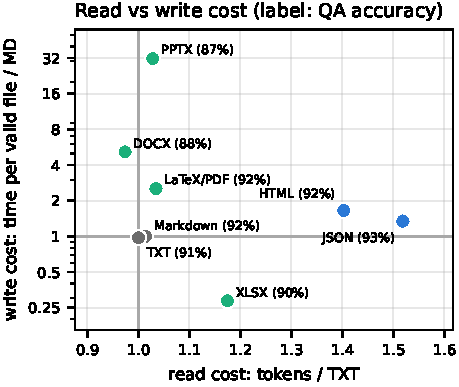
\includegraphics[width=\columnwidth]{figures_full/lifecycle.pdf}
\caption{Each file type for Qwen3-8B: read cost (tokens of its extracted
or marked-up text over TXT) against write cost (format tax). Labels give
full-document QA accuracy.}
\label{fig:lifecycle}
\end{figure}

Figure~\ref{fig:lifecycle} puts the two costs on one plot. Reading and
writing rank the formats differently. DOCX and PPTX are free to read once
their text is extracted, and the most expensive files to write. JSON and
HTML cost about 1.5$\times$ on both axes. Only TXT and Markdown cost about 1 on
both axes, and only Markdown keeps the headings, list and table. A PDF built from Markdown is nearly as cheap.
